\documentclass[12pt]{article}

\usepackage[utf8x]{inputenc}
\usepackage[english]{babel}

\usepackage{amssymb,amsmath,amsthm,amsfonts}
\usepackage{calc}
\usepackage{graphicx}
\usepackage[shortlabels]{enumitem}
\usepackage{subfigure}
\usepackage{gensymb}
\usepackage{float}
\usepackage{natbib}
\usepackage{url}
\usepackage[utf8x]{inputenc}
\usepackage{amsmath}
\usepackage{graphicx}
\graphicspath{{images/}}
\usepackage{parskip}
\usepackage{fancyhdr}
\usepackage{vmargin}
\usepackage{mathrsfs}
\usepackage{subfigure}
\usepackage[dvipsnames]{xcolor}
\usepackage{longtable}
\usepackage{multicol}
\usepackage{multirow}
\usepackage{booktabs}

%tikzpicture
\usepackage{tikz}
\usepackage{scalerel}
\usepackage{pict2e}
\usepackage{tkz-euclide}
\usetikzlibrary{calc}
\usetikzlibrary{patterns,arrows.meta}
\usetikzlibrary{shadows}
\usetikzlibrary{external}
\usepackage{listings}
\usepackage{xcolor}


\definecolor{lightgray}{rgb}{0.95,0.95,0.95}  % gris muy claro
% más oscuro:
% \definecolor{lightgray}{rgb}{0.9,0.9,0.9}
% aún más plomo:
% \definecolor{lightgray}{rgb}{0.85,0.85,0.85}

\lstset{
    language=C,
    basicstyle=\ttfamily\small,
    keywordstyle=\color{blue},
    commentstyle=\color{green!50!black},
    stringstyle=\color{red},
    numbers=left,
    numberstyle=\tiny,
    stepnumber=1,
    numbersep=5pt,
    frame=single,
    breaklines=true,
    tabsize=2
}
%pgfplots
\usepackage{pgfplots}
\pgfplotsset{compat=newest}
\usepgfplotslibrary{statistics}
\usepgfplotslibrary{fillbetween}

\setmarginsrb{3 cm}{2.5 cm}{3 cm}{2.5 cm}{1 cm}{1.5 cm}{1 cm}{1.5 cm}

\title{Homework 4}					% Titulo
\author{Matías I. Inostroza (mii2106)}					% Autor
\date{\today}						% Fecha


\makeatletter
\let\thetitle\@title
\let\theauthor\@author
\let\thedate\@date
\makeatother

\pagestyle{fancy}
\fancyhf{}
\rhead{\theauthor}
\lhead{\thetitle}
\cfoot{\thepage}

\begin{document}

%%%%%%%%%%%%%%%%%%%%%%%%%%%%%%%%%%%%%%%%%%%%%%%%%%%%%%%%%%%%%%%%%%%%%%%%%%%%%%%%%%%%%%%%%

\begin{titlepage}
	\centering
    \vspace*{0.0 cm}
    
\includegraphics[scale = 0.35]{Columbia_logo.png}\\[2.0 cm]	% Logo Universidad
    \textsc{\LARGE Columbia University}\\[2.0 cm]	% Nombre Universidad
	\textsc{\Large APMAE4302}\\[0.5 cm]				% Codigo Curso
	\textsc{\large Methods in computational science}\\[0.5 cm]		% Nombre Curso
	\rule{\linewidth}{0.2 mm} \\[0.4 cm]
	{ \huge \bfseries \thetitle}\\
	\rule{\linewidth}{0.2 mm} \\[1.5 cm]
	
	\begin{minipage}{0.4\textwidth}
		\begin{center} \large
			\emph{Author:}\\
			\theauthor\linebreak
			\end{center}
	\end{minipage}\\[2 cm]
	
	{May, 2026}\\[2 cm]
 
	\vfill
	
\end{titlepage}

%%%%%%%%%%%%%%%%%%%%%%%%%%%%%%%%%%%%%%%%%%%%%%%%%%%%%%%%%%%%%%%%%%%%%%%%%%%%%%%%%%%%%%%%%


\pagebreak

%%%%%%%%%%%%%%%%%%%%%%%%%%%%%%%%%%%%%%%%%%%%%%%%%%%%%%%%%%%%%%%%%%%%%%%%%%%%%%%%%%%%%%%%%
\section{Section 1}

The original equations are:

\vspace{-5mm}
\begin{eqnarray}
    \frac{\partial T}{\partial t} + \mathbf{v}\cdot \nabla T &=& \frac{1}{Ra}\nabla^2T\\
    -\nabla^2\mathbf{v} + \nabla p &=& T\mathbf{\hat{j}}\\
    \nabla\cdot \mathbf{v} &=& 0
\end{eqnarray}

\vspace{-5mm}

Let's define:

\vspace{-5mm}
\begin{eqnarray}
    \mathbf{v} = \nabla \times (\psi \mathbf{\hat{k}})\\ 
    \omega \mathbf{\hat{k}} = \nabla \times \mathbf{v}
\end{eqnarray}

First, the velocity is defined in terms of $\psi$ by writing the components explicitly:

\vspace{-5mm}

\begin{eqnarray}
   \mathbf{v} = \nabla \times\psi \mathbf{\hat{k}} =  \nabla \times(0,0,\psi) = (\frac{\partial \psi}{\partial y}, - \frac{\partial \psi}{\partial x},0)\\
   \rightarrow \nabla \cdot \mathbf{v} = \frac{\partial^2\psi}{\partial x \partial y} - \frac{\partial^2\psi}{\partial y \partial x} = 0
\end{eqnarray}

Thus, the incompressibility condition is automatically satisfied. Then, substituting (4) in (5)

\begin{equation}
    \omega \mathbf{\hat{k}} = \nabla \times (\nabla \times (\psi \mathbf{\hat{k}})) = \nabla(\nabla \cdot (\psi \mathbf{\hat{k}})) -\nabla^2( \psi \mathbf{\hat{k}} )
\end{equation}

Since the problem is two dimensional, that means $\psi(x,y)$ then $\nabla \cdot (\psi \mathbf{\hat{k}}) = \frac{\partial \psi}{\partial z} = \mathbf{0}$, and considering that $\mathbf{\hat{k}}$ is constant

\vspace{-5mm}

\begin{equation}
    \omega \mathbf{\hat{k}} = (-\nabla^2\psi) \mathbf{\hat{k}}
\end{equation}

And comparing the $\mathbf{\hat{k}}$ component, the third equation is obtained:

\vspace{-5mm}

\begin{equation}
    \omega = -\nabla^2\psi \textbf{ Answer.}
\end{equation}

From equation (2), applying $\nabla \times ()$ on both sides, and considering the identity $\nabla \times (\nabla a) = 0$, being $a$ a scalar field

\begin{eqnarray}
    -\nabla \times(\nabla^2 \mathbf{v}) + \nabla \times(\nabla p) = \nabla\times T\mathbf{\hat{j}} \\
        -\nabla \times(\nabla^2 \mathbf{v}) = \nabla\times T\mathbf{\hat{j}} 
\end{eqnarray}

The curl and Laplacian con commute, then, considering equation (5)

\vspace{-5mm}

\begin{eqnarray}
        -\nabla^2( \nabla \times\mathbf{v}) = \nabla\times T\mathbf{\hat{j}} \\
        -\nabla^2( \omega \mathbf{\hat{k}}) = \nabla\times T\mathbf{\hat{j}} 
\end{eqnarray}

\vspace{-3mm}

The right hand side $\nabla\times T\mathbf{\hat{j}} = (\frac{\partial T}{\partial z}, 0 , \frac{\partial T}{\partial x})$, but since the problem is two dimensional, then the variation of $T$ with respect to $z$ is zero, or $\frac{\partial T}{\partial z} = 0$. Also, $\mathbf{\hat{k}}$ is considered to be constant, then:

\vspace{-5mm}
\begin{eqnarray}
        -\nabla^2( \nabla \times\mathbf{v}) = \nabla\times T\mathbf{\hat{j}} \\
        -\nabla^2( \omega )\mathbf{\hat{k}} = \frac{\partial T}{\partial x} \mathbf{\hat{k}} 
\end{eqnarray}

\vspace{-5mm}
Comparing the $\mathbf{\hat{k}}$ component of the equation, second equation is obtained:

\vspace{-5mm}
\begin{eqnarray}
        -\nabla^2 \omega = \frac{\partial T}{\partial x} \textbf{ Answer.}
\end{eqnarray}


\section{Section 2} 

\textbf{a)} After running the three PETSc option files, Table 1 summarizes the results:

\begin{table}[h!]
\centering
\small
\begin{tabular}{lccccc}
\hline
\textbf{Options file} &
\textbf{SNES its} &
\textbf{KSP its} &
\textbf{SNES time (s)} &
\textbf{FLOPs} &
\textbf{Rate (Mflop/s)} \\
\hline
\texttt{direct}
& 1 & 1
& 4.0272
& $2.54\times10^8$
& 63 \\

\texttt{split\_direct}
& 1 & 1
& 5.2119
& $1.44\times10^8$
& 28 \\

\texttt{split\_mg}
& 1 & 7
& 3.8605
& $8.26\times10^8$
& 214 \\
\hline
\end{tabular}
\caption{Convergence and runtime comparison of PETSc solver configurations for the biharmonic problem.}
\label{tab:petsc_biharm}
\end{table}
All three PETSc configurations converged successfully. 
The direct and split-direct configurations required only one Krylov iteration because the linear systems were solved using direct LU factorization. 
The multigrid fieldsplit configuration required more Krylov iterations, but achieved the shortest solve time due to the efficiency of the multigrid preconditioner.

The \texttt{split\_mg} configuration also achieved the highest floating-point rate, indicating more efficient hardware utilization during the solve phase.
\newpage
\textbf{b)} After running the three option files with Firedrake, table 2 shows the results:


\begin{table}[h!]
\centering
\small
\begin{tabular}{lccccc}
\hline
\textbf{Solver option} &
\textbf{SNES its} &
\textbf{KSP its} &
\textbf{SNES time (s)} &
\textbf{FLOPs} &
\textbf{Rate (Mflop/s)} \\
\hline
\texttt{monolithic}
& 1 & 1 & 4.3293 & $2.11\times10^9$ & 488 \\
\texttt{fieldsplit\_direct}
& 1 & 1 & 3.2560 & $1.68\times10^9$ & 516 \\
\texttt{fieldsplit\_mg}
& 1 & 7 & 3.9000 & $2.58\times10^9$ & 661 \\
\hline
\end{tabular}
\caption{Convergence and runtime information for the Firedrake biharmonic solver configurations.}
\label{tab:firedrake_biharm}
\end{table}
All three Firedrake solver configurations converged successfully and produced comparable numerical solutions. 
The monolithic and \texttt{fieldsplit\_direct} configurations required only one Krylov iteration due to the use of direct LU factorization, while the multigrid configuration required more iterations but achieved competitive runtimes.

Among the tested configurations, \texttt{fieldsplit\_direct} achieved the lowest \texttt{SNESSolve} time, whereas \texttt{fieldsplit\_mg} achieved the highest floating-point rate at the expense of a larger number of FLOPs. 
Overall, the \texttt{fieldsplit\_direct} configuration provided the best balance between robustness and computational efficiency.


\textbf{c)}

\begin{table}[h!]
\centering
\small
\begin{tabular}{lcc}
\hline
\textbf{Quantity} & \textbf{PETSc C} & \textbf{Firedrake} \\
\hline
Mesh size & $513 \times 513$ & $512 \times 512$ \\

Solver configuration & \texttt{split\_direct} & \texttt{fieldsplit\_direct} \\

SNES iterations & 1 & 1 \\

KSP iterations & 1 & 1 \\

Total runtime (s) & 6.09 & 15.65 \\

SNESSolve time (s) & 5.21 & 3.26 \\

FLOPs & $1.45\times10^8$ & $1.68\times10^9$ \\

Rate (Mflop/s) & 28 & 516 \\

Relative error (vorticity) 
& $5.20\times10^{-5}$ 
& $5.72\times10^{-5}$ \\

Relative error (streamfunction) 
& $1.17\times10^{-4}$ 
& $1.46\times10^{-4}$ \\
\hline
\end{tabular}
\caption{Comparison between the PETSc C and Firedrake implementations using the direct fieldsplit solver configuration.}
\label{tab:c_vs_fd}
\end{table}

Both implementations converged successfully and produced comparable numerical errors. 
The PETSc C implementation achieved a significantly lower runtime, while Firedrake required substantially more floating-point operations.

The main difference arises from the discretization strategy and software framework used by each implementation. 
The PETSc C code uses a structured finite-difference discretization with low level assembly, whereas Firedrake employs finite elements, mixed function spaces, and automatically generated variational kernels, leading to larger algebraic and assembly costs.

Although Firedrake achieved a higher floating point rate, the larger computational workload dominated the runtime. 

Overall, both implementations produced similar numerical accuracy, but the PETSc C implementation was computationally more efficient for this benchmark problem.

\section{Section 3} For this part, the following modifications were introduced to the original \texttt{biharm.py} code, including the definition of the temperature field ass:

\begin{equation}
    T(x,y) = (1-y) + A\cos(\pi x)
\end{equation}

And a RHS function as:

\begin{equation}
    f(x) = \frac{\partial T}{\partial x}
\end{equation}

\begin{lstlisting}
A = 0.1
T = Function(V,name="Temperature")
T.interpolate((1.0-z)+A*cos(pi*x))
f.interpolate(T.dx(0))
\end{lstlisting}

No error analysis was performed for this part, since the problem is not posed as a manufactured solution test. Instead, the objective is to use the prescribed temperature field to compute the forcing term $f=\partial T/\partial x$ and solve the corresponding biharmonic streamfunction vorticity system. Therefore, the result is assessed qualitatively through the Paraview visualization of the temperature field, streamfunction contours, and velocity field.

Figure 1 shows the temperature field with the stream function as contour plot (most likely circle shaped), and the velocity vectors in grey color.

\newpage
\begin{figure}[htbp]
    \centering
    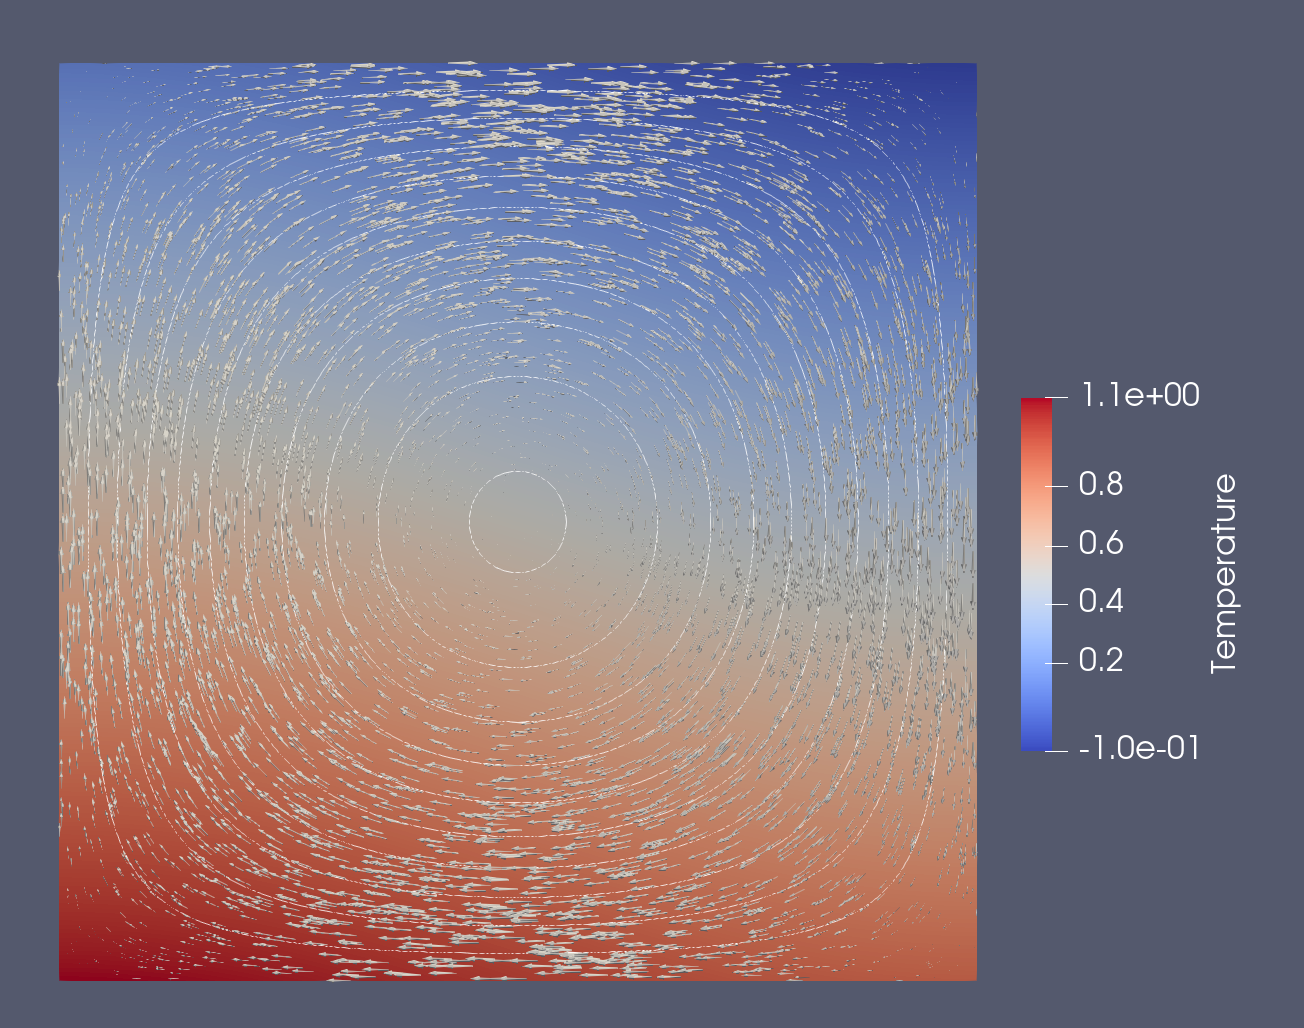
\includegraphics[width=0.6\textwidth]{Figures/3.png}
    \caption{Solution from Firedrake}
    \label{fig:knn-accuracy}
\end{figure}

\section{Section 4}
Starting from the temperature equation

\begin{equation}
\frac{\partial T}{\partial t}
+
\mathbf{v}\cdot\nabla T
=
\frac{1}{Ra}\nabla^2 T
\end{equation}

the equation is multiplied by a test function $q$ and integrated over the domain $\Omega$:

\begin{equation}
\int_\Omega
q \frac{\partial T}{\partial t}\, d\Omega
+
\int_\Omega
q\, \mathbf{v}\cdot\nabla T\, d\Omega
=
\frac{1}{Ra}
\int_\Omega
q\, \nabla^2 T\, d\Omega
\end{equation}

Integrating the diffusion term by parts gives

\begin{equation}
\int_\Omega
q \frac{\partial T}{\partial t}\, d\Omega
+
\int_\Omega
q\, \mathbf{v}\cdot\nabla T\, d\Omega
+
\frac{1}{Ra}
\int_\Omega
\nabla q \cdot \nabla T\, d\Omega
=0
\end{equation}

where the boundary integral vanishes due to the prescribed boundary conditions.

Therefore, the weak form used in the Firedrake implementation is

\begin{equation}
F_T(T;q)
=
\int_\Omega
q\, T_t\, d\Omega
+
\int_\Omega
q\, \mathbf{v}\cdot\nabla T\, d\Omega
+
\frac{1}{Ra}
\int_\Omega
\nabla q \cdot \nabla T\, d\Omega
\end{equation}

This is the line code implemented in firedrake

\begin{lstlisting}
FT = (q*T_dot*dx+ q*dot(vel, grad(T))*dx + (1.0/Ra)*inner(grad(T), grad(q))*dx)
\end{lstlisting}
\textbf{a)} The boundary conditions were implemented as:

\begin{lstlisting}
bcs = [DirichletBC(ME.sub(0), 1.0, 3),   # T(x,0,t)=1
       DirichletBC(ME.sub(0), 0.0, 4),   # T(x,1,t)=0
       DirichletBC(ME.sub(1), 0.0, "on_boundary"),  # omega=0
       DirichletBC(ME.sub(2), 0.0, "on_boundary"),  # psi=0]
\end{lstlisting}

And for computation of the Nusselt number, the following equation was implemented:

\begin{equation}
    Nu = -h\frac{\int_0^l\partial_z T(x, z=h)dx}{\int_0^l T(x, z=0)dx}
\end{equation}

with $h=1$. This definition was taken from Lecture 20. Unfortunately, the expression provided in the homework statement did not produce reasonable values of the Nusselt number greater than 1. Using the homework definition, the computed value of $Nu$ always converged to approximately 1, and I could not figure out the error.

Figure 2 shows the Nusselt number for $Ra = 10^2$.

\begin{figure}[htbp]
    \centering
    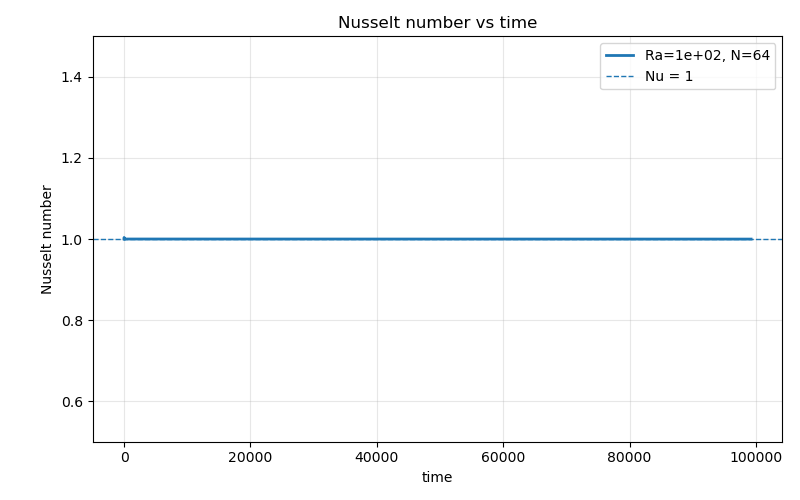
\includegraphics[width=0.75\textwidth]{Figures/4a.png}
    \caption{Nusselt number for $Ra = 10^2$}
    \label{fig:knn-accuracy}
\end{figure}

For $Ra=10^2$ on a $64\times64$ Q1 mesh, the computed Nusselt number converged to $Nu \approx 1$

Since the Nusselt number measures the total heat flux relative to the purely conductive heat flux, $Nu=1$ indicates that heat transport is dominated by conduction and that there is no significant convective enhancement. Therefore, the steady state for $Ra=10^2$ is non convective.

\textbf{b)} For larger Rayleigh numbers, the evolution of $Nu$ is shown in Figure 3. The final values of $Nu$ at $t=100000\ \text{s}$ are reported in Table 4.

\begin{figure}[htbp]
    \centering
    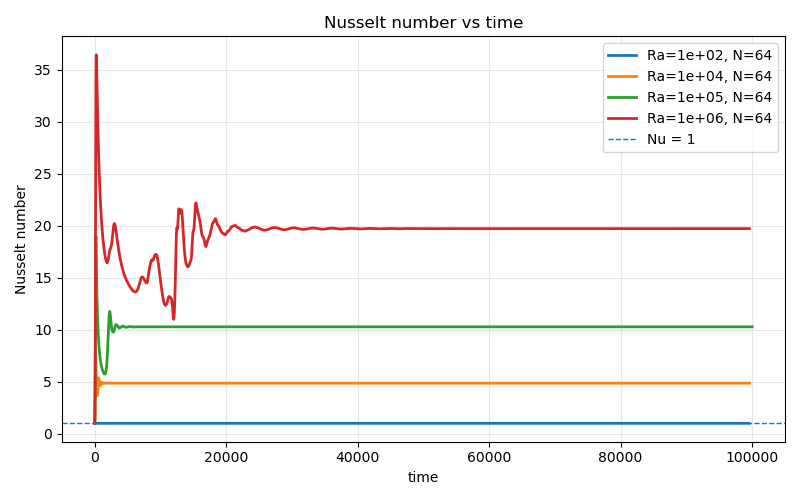
\includegraphics[width=0.75\textwidth]{Figures/4b.png}
    \caption{$Ra$ analysis}
    \label{fig:knn-accuracy}
\end{figure}

\begin{table}[h!]
\centering
\caption{Final Nusselt number for different Rayleigh numbers using a $64\times64$ mesh.}
\begin{tabular}{cc}
\hline
Rayleigh Number ($Ra$) & Final Nusselt Number ($Nu$) \\
\hline
$10^2$ & 0.999 \\
$10^4$ & 4.859 \\
$10^5$ & 10.274 \\
$10^6$ & 19.711 \\
\hline
\end{tabular}
\label{tab:nusselt_results}
\end{table}


\newpage

 \textbf{c)} Figure 4 shows the mesh convergence of the final Nusselt number for $Ra=10^4$. 
As the mesh is refined from $16\times16$ to $128\times128$, the computed value of $Nu$ increases and approaches the Blankenbach benchmark value $Nu=4.884$. 
The coarse $16\times16$ mesh underestimates the heat flux, while the $64\times64$ and $128\times128$ meshes give values very close to the benchmark. 
This indicates that the numerical solution is converging with mesh refinement.

\begin{figure}[htbp]
	\centering
	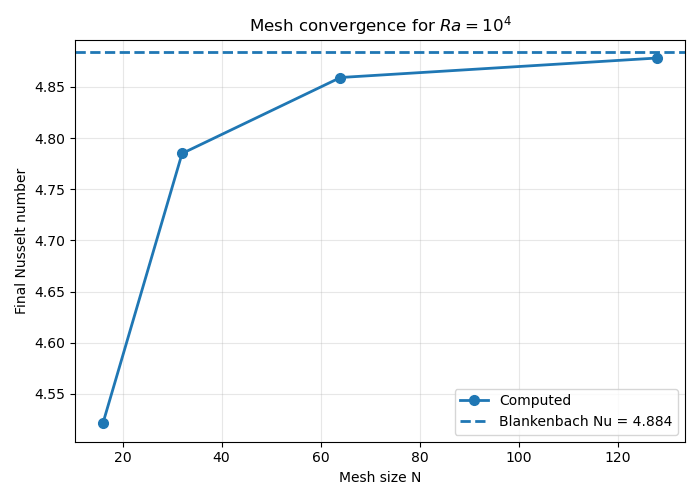
\includegraphics[width=0.75\textwidth]{Figures/4c.png}
	\caption{Convergence analysis}
	\label{fig:knn-accuracy}
\end{figure}
\end{document}
